\documentclass[11pt]{article}

\usepackage[UTF8]{ctex} % for Chinese 

\usepackage{setspace}
\usepackage[colorlinks,linkcolor=blue,anchorcolor=red,citecolor=black]{hyperref}
\usepackage{lineno}
\usepackage{booktabs}
\usepackage{graphicx}
\usepackage{float}
\usepackage{floatrow}
\usepackage{subfigure}
\usepackage{caption}
\usepackage{subcaption}
\usepackage{geometry}
\usepackage{multirow}
\usepackage{longtable}
\usepackage{lscape}
\usepackage{booktabs}
\usepackage{natbib}
\usepackage{natbibspacing}
\usepackage[toc,page]{appendix}
\usepackage{makecell}

\title{老子}
\date{}

\linespread{1.5}
\geometry{left=2cm,right=2cm,top=2cm,bottom=2cm}

\begin{document}

  \maketitle
  
  \begin{figure}[H]
    \centering
    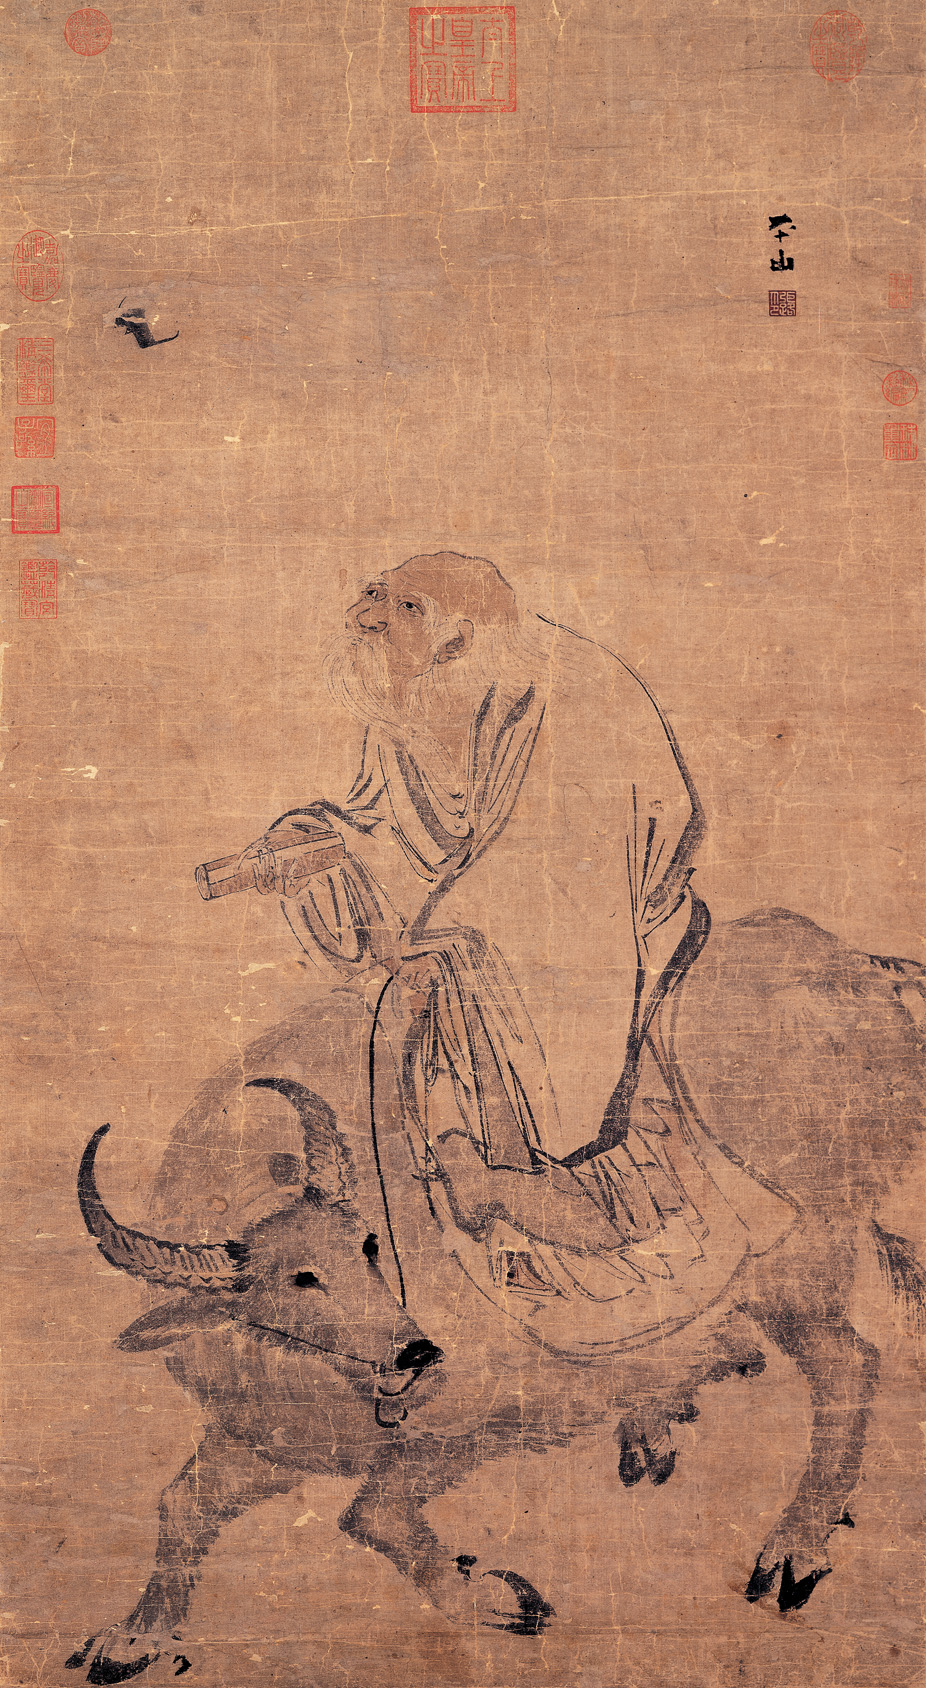
\includegraphics[height=0.7\textwidth]{../Figures/LaoZi.jpg}
    \caption{老子像。台湾国立故宫博物院藏。}
  \end{figure}

  \newpage
  
  \linenumbers

老子姓李名耳,楚之苦县人,早年任周之小吏,管理藏书。
孔子曾问礼于老子,对其异常倾佩,以为人中龙凤。
后老子云游四方,遍观人间疾苦,悟得大道,遂西出函谷,行将飞升。
关令尹喜恐老子隐后,大道不传,强留其著书。
老子遂作《道德经》五千言遗之,而后一路西行。
途径戎狄之国,见其民堕于外道邪法,甚悲悯之。遂举大神通,欲化之以正法大道。
又恐夷民粗鄙愚笨,难解大道,遂作浮屠之法传之。
有戎国王子乔达摩·悉达多,得老子牙慧,竟成佛陀,其学显赫至今。
而老子深藏功名,拂衣而去,羽化飞升。
今人所供奉之太上老君,即是老子。

\newline

以上所述老子生平出自民间传说,基本属于虚构,但“深藏功名,拂衣而去”,却非妄言。
老子系中国文化一甚大人物。
据说世界各类图书的销量榜单上,《道德经》排进前三,且各种乱七八糟的译本层出不穷。
汉代道教兴起后,老子更是坐上了全宇宙第一把交椅。
然此等显赫人物,竟神龙见首不见尾,其身世、时代皆成问题,就连姓名亦存疑窦。
老子其书其人,真伪先后之辩,积讼已久,历代学者群言兹繁,鲜有一较为确定之结论。
写出这般作品却不署名,可见其不为名利所绊,真真天下第一潇洒人物。
不信,试观今日,哪位敢写篇东西不注明作者、声明版权所有?
连我这种没受过教育的货色写篇小论文,尚且要写清楚作者是谁,甚至还要注明所属单位,免得和别人重名,引发误会。
想到老子之境界,再看看自己,真愧煞人也。
  
  道
  万物流变不息,皆不能久常。《道德经·二十三章》谓:
  飘风不终朝,骤雨不终日。孰为此者?天地。天地尚不能久,而况於人乎?
  换言之,凡属于客观物质世界者,皆处于一不断变化之状态。而万物所依循之规律,系一超出物质世界之存在,故可久可常。此种规律,老子名之曰“道”。
  道为万物之形成、流变所依恃之规律,系一超越万物之独立存在,而非万物之一。此规律之运行,遍于万物而无终止。道对物质世界起一范铸作用,物质世界依照道来运行,而非万物起源于道这一超越存在,亦非道于时间顺序上先于万物存在。
  道系万物之总原理,故不可言说。盖可以语言描述之规律,势必有其作用范围。换言之,可言说之原理,其作用范围必为某类事物;而道之作用范围为一切事物。故无法对道作正面诠释,言其是什么;而只能作否定性断语,即道不是什么。换言之,道而非具体事物,故不能以具体事物或形容具体事物之名来指代或形容道。盖凡命名,系由一组条件限定范围,遂有“此”和其反面“非此”之区分。而道之运行遍在于万物,无从为之限定范围,无从寻其反面,故道无名,不可正面定义。《道德经·一章》载:
  道可道,非常道;名可名,非常名。
  道之内容为反。《道德经·四十章》云:
  反着道之动。
  每一事物或性质均有其反面。事物发展至于某一极端,则必然向另一相反极端逐渐转变,此即所谓“反”。“动”指运行。故“反”为道之运行表现,为道范铸万物之表现,为道之效用。换言之,“反”之于“道”,乃一充分性概念,而无必要性,故不可将二者等同。
  
  无为
  万物流变,悉在变逝之中,皆无实性,故皆为不可凭依者。由此老子主张无为,即自觉心不陷溺于任何外在事物。事物均在“反”中,故不可执,执则必为陷溺。心合于道,观万物于反中变逝,而自觉不陷溺于物,此即无为之境界。换言之,自觉心不依靠任何客观事物,方能超越万物,达到道之境界,遂观万殊事物之永恒理序。
  自觉心脱离乃至于超越客观事物,达到无为之境界,得知大道之本质,朗照万物之根本。由此延伸,易得佛家舍离之说。通晓“道”之自觉心,已然超越万物,独立于物质世界,即所谓“跳出三界外,不在五行中”,则人之自觉脱离物质世界乃一自然而然之结论。济癫僧之“修心不修口”,便是此类观点。盖自觉心已达超越万物之无为境界,彻底脱离物质世界,而作为万物之一的躯体不过自觉心一载体,修口已无意义矣。佛学初入中国,假称老子化胡为佛,便是基于老子理论中此种倾向,以便于传播。
  然而老子并未走向舍离之说。依照老子,自觉心既升入超越之境界,朗照万物,遂可由中生出对客观物质世界之支配力,即由无为生出实用主张,所谓“无为而无不为”。换言之,佛欲以自觉心之超越性脱离物质世界之束缚,而老子欲以此支配物质世界。后世道教致力于采药炼丹、钻研方术、探究医理,追求长生不老、白日飞升、羽化成仙,与老子不无干系。
  
  守柔
  现论无为之实用价值。无为之终极目的在于观道,则其延伸实用主张亦以道为依据。道之内容曰反,故老子之实用主张亦以反为根基,可概括为“守柔”。
  老子谓柔能胜强,故守柔方为真正强大。《道德经·七十六章》谓:
  人之生也柔弱,其死也坚强。草木之生也柔脆,其死也枯槁。故坚强者死之徒,柔弱者生之徒。是以兵强则灭,木强则折。强大处下,柔弱处上。
  柔弱之支配力,其依据在于反。万物依道运行,时时皆反,故一切存在皆处于自身否定之过程中。事物发展至极点,不可避免要变为其反面。故人若自恃勇力,无论其力量如何强大,其运用结果必然是走向衰弱。而自守柔弱,即预先居于强大之反面,自然逐渐强大而不至于衰竭。一言以蔽之,人若欲如何,必先居于此如何之反面,南辕正所以取道北辙,欲强大则需守柔弱,欲擒之则需先纵之。《道德经·三十六章》载:
  将欲歙之,必故张之;将欲弱之,必故强之;将欲废之,必故兴之;将欲取之,必故与之。是谓微明。柔弱胜刚强。鱼不可脱於渊,国之利器不可以示人。
  总而言之,老子所推崇之人生态度为把握万物所依之道而支配万物,且此种支配力量为一自然而然产物,非勉强为之。境界至高之人,其自觉心超乎物质世界,与朗照万物之“道”平齐,不溺陷于外在事物,通彻“反”之原理,自守柔弱之地位,于物质世界有不竭之支配力量。此为一自然而然之境界,无需钻营图谋。
  老子常以婴儿比喻此等至人。《道德经·五十五章》载:
  含德之厚,比于赤子。
  有大智慧之人,依照物极必反之原理,往往看似愚笨,如婴儿般无知,此即所谓大智若愚。而今人以老子之理论从事阴谋,进而将《道德经》视为兵法韬略,用于钻营者非为少数。此实陷溺于外物,大悖老子之学。
  
  政治理论
  物极必反之原理,其影响亦见诸老子之政治理论。若欲使国家得治而精心设计各种制度、构建官僚体系、编撰律法政令,如此钻营,终将产生与原目的相反之结果。换言之,国家之混乱,其根源在于政治秩序,在于社会、文化之发展。唯有尽数破之,方能使国家承平。故《道德经·五十七章》云:
  天下多忌讳,而民弥贫;人多利器,国家滋昏;人多伎巧,奇物滋起;法令滋彰,盗贼多有。故圣人云:“我无为,而民自化;我好静,而民自正;我无事,而民自富;我无欲,而民自朴。”
  老子视万有为变逝之物象,遂不肯定任何特殊规范、秩序,亦不肯定知识、文化之价值。由此,其所肯定者乃所否定者之反面。《道德经·三章》载:
  是以圣人之治,虚其心,实其腹,弱其志,强其骨。常使民无知无欲。使夫智者不敢为也。
  老子所谓圣人之治,系否定知识文化,使民众保持婴儿之天真纯朴,即欲愚民。前述圣人亦愚,却是大智若愚之愚,为至高境界之返璞归真,系修养所成之境界。而一般民众之愚,是人生来之淳朴无知。老子谓圣人治国,当使民众安于本来之愚,免于被文化知识扰乱。至于政治制度,更是余食赘形。
  综上,遂有老子之理想社会蓝图,见诸《道德经·八十章》:
  小国寡民。使有什伯之器而不用;使民重死而不远徙;虽有舟舆,无所乘之;虽有甲兵,无所陈之。使人复结绳而用之。至治之极。甘其食,美其服,安其居,乐其俗,邻国相望,鸡犬之声相闻,民至老死不相往来。
  此一蓝图,绝非开历史的倒车,退回原始社会。“什伯之器”、“舟舆”、“甲兵”皆有而不用,况又能“甘其食,美其服,安其居,乐其俗”,此非原始社会之野蛮状况,而为包含野蛮之文明境界。以物极必反之原理,此为“大文明若野蛮”也,是社会发展至终极,抛弃无价值之体制、文化,人民淳朴豁达、安居乐业之最高境界。
  
  自我境界
  老子之自我境界殊不易解,其原因在于老子论及此类问题,所否定者多,所肯定者少。今兹立一标准,以推测老子之自我境界。
  自我境界可分为四个层次。形躯,即人之物质欲求,诸如欲观美色、听天籁、尝美食等。认知,即人之推理活动以及对客观事物之研究和理解,为人之理性。此素为西方哲学所重视,亦为数理逻辑和自然科学所依附。德性,即人之道德意识和价值自觉,为孔孟所重视者。情意,即生命力和生命感,为人之感性,系一观赏之境界、艺术之境界、美学之境界。
  首先,老子否定形躯。《道德经·十二章》载:
  五色令人目盲;五音令人耳聋;五味令人口爽;驰骋畋猎,令人心发狂;难得之货,令人行妨。是以圣人为腹不为目,故去彼取此。
  此章否定形躯欲求之满足,谓之为有害无益。盖形躯亦为万物之一,故亦循道而行。倘为求养生而满足欲望,追求“五色”“五音”“五味”,只会得到相反之结果,反而害生。故圣人养生,只满足生活之基本需求而不溺于物质欲求。
  其次,老子否定德性。《道德经·十八章》谓:
  大道废,有仁义;智慧出,有大伪;六亲不和,有孝慈;国家昏乱,有忠臣。
  《道德经·三十八章》更是抨击仁义礼智诸德:
  故失道而后德,失德而后仁,失仁而后义,失义而后礼。夫礼者,忠信之薄,而乱之首。
  德、仁、义皆为失道后逐步堕落之产物,而礼更是堕落之极致。由此,老子对德性之否定已甚明显矣。
  再次,老子否定认知,视知识、技术、文化为堕落。《道德经·五十七章》云:
  天下多忌讳,而民弥贫;人多利器,国家滋昏;人多伎巧,奇物滋起;法令滋彰,盗贼多有。
  引文不仅否定自然科学和技术,连社会文化、制度一并否定。《道德经·六十五章》又载:
  古之善为道者,非以明民,将以愚之。民之难治,以其智多。故以智治国,国之贼;不以智治国,国之福。
  此节否定“智”,直言其为国贼。可见,老子否定认知。
  至此,形躯、德性、认知皆被否定。依前述标准,可推测老子所肯定为人之情意。此一点老子鲜有明言,然观老子盛赞婴儿之生命力,与肯定情意之倾向一致。《道德经·五十五章》谓:
  含德之厚,比於赤子。毒虫不螫,猛兽不据,攫鸟不搏。骨弱筋柔而握固。未知牝牡之合而朘作,精之至也。终日号而不嘎,和之至也。知和曰常,知常曰明。益生曰祥。心使气曰强。物壮则老,谓之不道,不道早已。
  由此可初步下一结论,老子所肯定之自我,乃人之情意。


\end{document}